\documentclass[logo,reportComp]{thesis}
\usepackage[cpp,pseudo,optidef]{mypackage}

\title{高级编程技术期末大作业}
\subtitle{天池新人赛:快来一起挖掘幸福感!}
\school{数据科学与计算机学院}
\author{
陈鸿峥$^\star$\qquad\quad 冯家苇$^\star$\qquad\quad \makebox[3em][s]{符\hspace{\fill}尧}$^\star$\qquad\quad \makebox[3em][s]{傅\hspace{\fill}畅}\protect\footnote{以学号为序,不代表贡献大小}\qquad\quad\\17341015\qquad 17341035\qquad 17341037\qquad 17341038}
\classname{17计算机科学与技术}
\stunum{}
\headercontext{高级编程技术期末大作业}
\lstset{language=python}

\begin{document}

\maketitle

\section{题目描述}
幸福感与每个人息息相关,每个人对幸福感都有自己的衡量标准。如果能发现影响幸福感的共性,生活中是不是将多一些乐趣;如果能找到影响幸福感的政策因素,便能优化资源配置来提升国民的幸福感。

故本赛题\footnote{阿里巴巴天池大赛-【新人赛】 快来一起挖掘幸福感!\url{https://tianchi.aliyun.com/competition/entrance/231702/information}}将利用调查问卷得到的数据对人们的幸福感进行预测。
本赛题使用的数据来自中国人民大学中国调查与数据中心主持之《中国综合社会调查(CGSS)》项目,其中的变量包括个体变量(性别、年龄、地域、职业、健康、婚姻与政治面貌等等)、家庭变量(父母、配偶、子女、家庭资本等等)、社会态度(公平、信用、公共服务等等)等,通过这些指标来预测人们对于幸福感的评价。

输入文件说明:
\begin{itemize}
	\item \verb'complete'文件为变量完整版数据
	\item \verb'abbr'文件为变量精简版数据
	\item \verb'index'文件中包含每个变量对应的问卷题目,以及变量取值的含义
	\item \verb'survey'文件是数据源的原版问卷,作为补充以方便理解问题背景
\end{itemize}

提交结果为\verb'csv'文件,其中包含\verb'id'和\verb'happiness'的预测值两列。
注意\textbf{预测值可以不为整数}。
评价指标为均方误差(MSE)
\[MSE=\frac{1}{n}\sum_{i=1}^n(y_i-\hat{y}_i)^2\]
其中,$n$为测试集样本数,$y_i$为第$i$个样本的真实值,$\hat{y}_i$为第$i$个样本的预测值。

\section{数据清洗}
由于完整数据集包含140个指标,每个指标的内容及表示方法都不同,因此读入数据后的第一步是进行数据清洗。
涉及以下几个方面:
\begin{itemize}
	\item 变量的编码:如出生年份是一个连续型变量(从1921年到1997年连续变化),而城市属于离散型变量(不同城市之间只是编号不同,但城市编号不反映大小关系)。
	\item 缺失数据的填充:因为各种原因,人们在填写调查问卷时总会缺失一些信息,或者因为调查问卷本身的设计导致调查者不需要填写某一指标。但对于数据分析来说,不同样本的维度不同是很难处理的,因此需要把这些缺失的信息用合理的数据填充上去。
	\item 特征的选择:并非所有指标都对我们的幸福感预测有用,如调查时间存在非常强的随机性且明显与幸福感无关故可以直接删除。而有些指标相互之间存在强相关关系,那么可以只保留一个进行分析。
\end{itemize}

\subsection{负数数据处理}
将含有负数的表项按照含义置为0或\verb'NaN'(Not a Number),举例如下所示
\begin{lstlisting}
data.loc[data['income'] < 0, 'income'] = 0
data.loc[data['join_party'] < 0, 'join_party'] = np.nan
\end{lstlisting}

\subsection{创造新特征}
相比起受访者受教育的年份,我们可能更在意受访者受教育的年龄,所以我们需要对这些数据进行处理(简单的计算),进而创造出新的特征,如下
\begin{lstlisting}
data['edubir'] = data['edu_yr'] - data['birth']
\end{lstlisting}

其他如收入比率、家庭收入占比等可以通过现有数据计算出来的,也应先计算出来,如下
\begin{lstlisting}
data['income/family_income'] = data['income'] / (data['family_income'] + 1)
data['all_income/family_income'] = (data['income'] + data['s_income']) / (data['family_income'] + 1)
\end{lstlisting}

一些数据均值也可以先计算出来,如下
\begin{lstlisting}
data['province_income_mean'] = data.groupby(['province'])['income'].transform('mean').values
\end{lstlisting}

完整的数据处理过程请见代码文件。

\subsection{归一化处理}
将新的特征和原有的特征进行整合,并进行归一化,防止数据之间差异太大。
\begin{lstlisting}
min_max_scaler = MinMaxScaler()
X_train = min_max_scaler.fit_transform(X_train)
\end{lstlisting}

\section{模型搭建}
本次比赛我们采用了集成学习(ensemble learning)的方法,采用五个子模型(岭回归、支持向量回归、三种梯度提升方法),最后采用一个线性模型(贝叶斯岭回归)对这五个子模型的预测效果进行整合。

由于最终评价指标是MSE,故我们所有的模型都是回归模型,主要优化下面这条最小二乘表达式
\begin{mini*}
{\vw}{\norm{X\vw-\vy}_2^2}{}{}
\end{mini*}
其中$X=\bmat{\vx_1 & \cdots & \vx_n}^\T$为样本特征的集合,$\vw$为需要训练的权重(注意这里为了表达方便,将偏置量$\vb$也融入其中),$\vy$为真实幸福感指数。

\subsection{RidgeRegression}
岭回归(Ridge Regression)即在原式的基础上添加一个L2正则化项(令$\vw$的各项元素之间差距不会太大),使得优化目标变为
\begin{mini*}
{\vw}{\norm{X\vw-\vy}_2^2+\lambda\norm{\vw}_2^2}{}{}
\end{mini*}

通过求梯度可以解得显式解
\[\vw=(X^\T X+\lambda I)^{-1}X^\T\vy\]

\subsection{SVR}
支持向量回归(Support Vector Regression, SVR)则是在岭回归的基础上添加一个边界范围。
\begin{mini*}
{\vw}{\frac{1}{2}\norm{\vw}_2^2}{}{}
\addConstraint{-\eps \leq y_i-\vx_i^\T\vw\leq\eps}{,\;\forall i}
\end{mini*}

通过求拉格朗日函数及拉格朗日对偶问题,同样可以得到迭代解法。

\subsection{XGBoost}
XGBoost即eXtreme Gradient Boosting,最早由华盛顿大学陈天奇提出,作为现在数据挖掘比赛中的利器,也被使用到我们的模型中。

首先阐述梯度提升(gradient boosting)这一集成学习常用方法的思想。
即对目标函数$f(\vx)$进行多次逼近,通过不断拟合残差达到逼近的效果,可以按照下式不断迭代
\[\begin{aligned}
f_1(\vx) &=\widehat{f}(\vx)            & h_1(\vx) &=f(\vx)-f_1(\vx)\\
f_2(\vx) &=f_1(\vx)+\widehat{h_1}(\vx) & h_2(\vx) &=f(\vx)-f_2(\vx)\\
f_3(\vx) &=f_2(\vx)+\widehat{h_2}(\vx) & h_3(\vx) &=f(\vx)-f_3(\vx)\\
\vdots   &                             & \vdots \\
f_n(\vx) &=f_{n-1}(\vx)+\widehat{h_{n-1}}(\vx)
\end{aligned}\]

对于最小二乘问题,负梯度就是每次计算得到的残差。
由于每次都新增一个残差项,因此被称为梯度提升。
% https://medium.com/@cwchang/gradient-boosting-%E7%B0%A1%E4%BB%8B-f3a578ae7205

而回归/决策树(decision tree)则是每次选择信息增益最大/基尼指数最小的特征作为结点进行划分,最终形成一棵树,每次预测时根据树结点的判断寻找对应的叶结点,即得到最终的预测值。

将梯度提升和决策树结合起来就得到梯度提升回归树(Gradient Boosting Regression Tree, GBRT),其核心在于,它的每棵树都是从上一次训练的所有树的残差中进行学习,进而拟合一棵回归/分类树,如图\ref{fig:tree-ensemble}所示。
\begin{figure}[H]
\centering
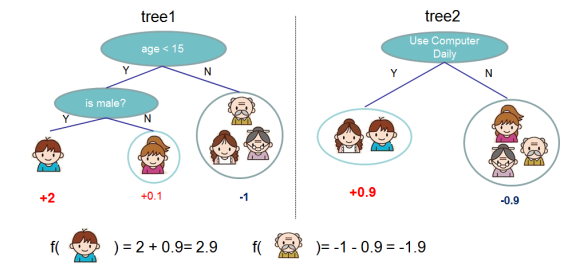
\includegraphics[width=0.5\linewidth]{fig/tree-ensemble.png}
\caption{树集成模型,图源自XGBoost原始论文}
\label{fig:tree-ensemble}
\end{figure}
故对于这一模型而言,其预测值就是
\[\hat{y}_i=\sum_{k=1}^Kf_k(\vx_i)\]

有目标优化问题
\begin{mini*}
{}{\sum_i l(y_i,\hat{y}_i)+\sum_k\Omega(f_k)}{}{}
\end{mini*}
其中,$l$为损失函数(loss),$\Omega$为每棵树的复杂度,为惩罚项。

通过对目标函数进行Taylor展开并求梯度,可以得到迭代更新的表达式,具体请见XGBoost的原始论文。

相比起传统的GBRT,XGBoost的优势在于以下几点:
\begin{itemize}
	\item 传统GBRT只用了一阶梯度信息,而XGBoost采用了二阶Taylor展开,精度更高
	\item XGBoost在目标函数中添加了正则化项,用于控制模型的复杂度
	\item 通过在迭代式中添加一个缩减(shrinkage)项(类似于学习率),防止越过最优解,同时防止过拟合
	\item 并行化处理
\end{itemize}

% ID3、C4.5、CART、随机森林、bagging、boosting、Adaboost、GBDT、xgboost算法总结 - yuyuqi的文章 - 知乎 https://zhuanlan.zhihu.com/p/34534004

\subsection{LightGBM}
之后的几种梯度提升方法都可以看作是对XGBoost的一种改进。

LightGBM是微软提出的一种高效的大规模并行梯度提升的框架,其相比于XGBoost又有以下几点改进:
\begin{itemize}
	\item 更快的训练速度和更高的效率
	\item 更低的内存占用
	\item 更高的准确率
\end{itemize}

这些都源于其采用了leaf-wise的决策树增长方式,而不是level-wise的增长方式,如图\ref{fig:tree-growth}所示。
\begin{figure}[H]
\centering
\begin{tabular}{c}
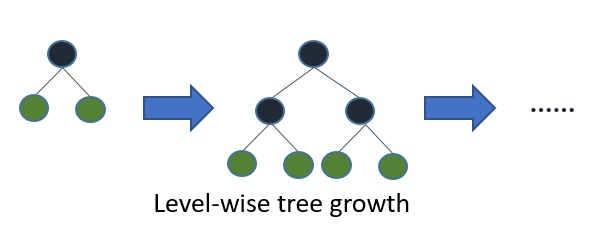
\includegraphics[width=0.6\linewidth]{fig/level-wise.jpg}\\
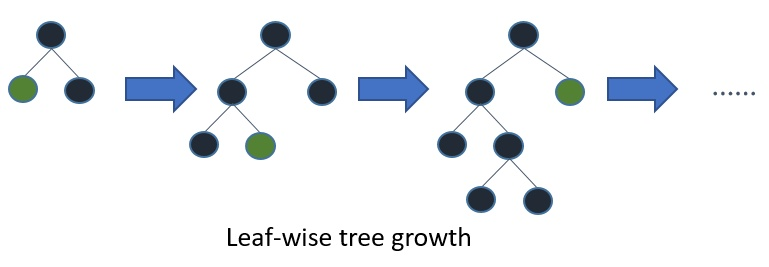
\includegraphics[width=0.6\linewidth]{fig/leaf-wise.jpg}
\end{tabular}
\caption{不同的树增长方式}
\label{fig:tree-growth}
\end{figure}

\subsection{CatBoost}
CatBoost则是俄罗斯Yandex公司提出的梯度提升框架。

传统GBDT算法通常对特征进行独热编码(ont-hot encoding)后进行训练。
而CatBoost则对离散型变量进行特殊的处理,先将样本随机排序,然后选取前$p-1$个样本做平均$y$值代替,同时加入了$a$和$P$作为超参数进行平衡,如下
\[\frac{\sum_{j=1}^{p-1}[x_{\sigma_j,k}=x_{\sigma_p,k}]Y_{\sigma_j}+a\cdot P}{\sum_{j=1}^{p-1}[x_{\sigma_j,k}=x_{\sigma_p,k}]+a}\]

CatBoost还结合上述样本排序方法,采用了一种新的计算方法来生成树结构,可以有效缓解过拟合。

% 作者:金世泳
% 链接:https://zhuanlan.zhihu.com/p/67794789

\subsection{BRR}
最后一个模型则是贝叶斯岭回归(Bayesian Ridge Regression),将前面五个模型的预测值再做一次回归分析。

五个子模型的预测值相当于贝叶斯回归中的取样结果,即用先验分布推后验分布,最终得到更为精确的拟合曲线。


\section{具体实施}
由于比赛方没有提供验证集,故对于每一个子模型,我们都采用\emph{K折交叉验证}的方法,将数据集划分为$k$等分,其中$k-1$份用于训练,剩下一份用于验证。

这里只截取最后一个综合模型(\verb'BayesianRidge')的代码,其他模型实现方法类似,请见源文件。
\begin{lstlisting}
train_stack = np.vstack([oof_lgb, oof_xgb, oof_cb, oof_svr, oof_rig]).transpose()
test_stack = np.vstack([predictions_lgb, predictions_xgb, predictions_cb, predictions_svr, predictions_rig]).transpose()

folds_stack = RepeatedKFold(n_splits=5, n_repeats=2, random_state=4590)
oof_stack = np.zeros(train_stack.shape[0])
predictions = np.zeros(test_stack.shape[0])

for fold_, (trn_idx, val_idx) in enumerate(folds_stack.split(train_stack, target)):
    print("fold {}".format(fold_))
    trn_data, trn_y = train_stack[trn_idx], target.iloc[trn_idx].values
    val_data, val_y = train_stack[val_idx], target.iloc[val_idx].values

    clf_3 = BayesianRidge()
    clf_3.fit(trn_data, trn_y)

    oof_stack[val_idx] = clf_3.predict(val_data)
    predictions += clf_3.predict(test_stack) / 10
\end{lstlisting}

\section{实验结果}
\subsection{结果分析}
\textcolor{red}{插几张数据结果图,简单分析一下}


\subsection{最终排名}
我们修改了不同的超参数,提交了两个版本,都取得了不错的成绩,如图\ref{fig:ranking}所示。
\begin{figure}[H]
\centering
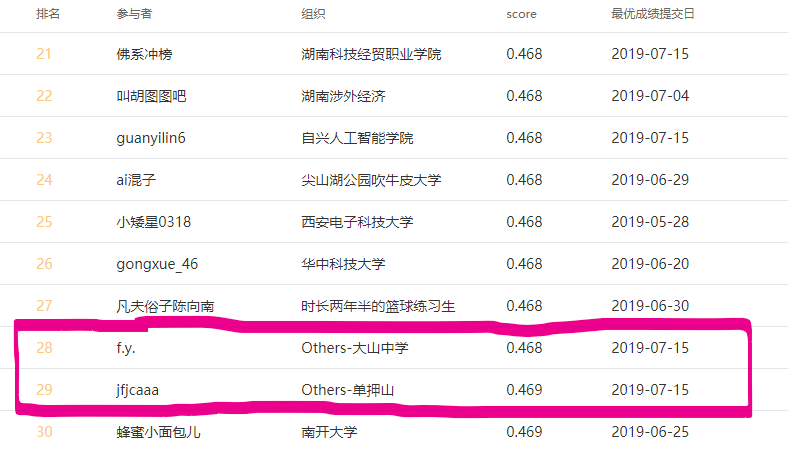
\includegraphics[width=0.7\linewidth]{fig/ranking-2.png}
\caption{最终成绩}
\label{fig:ranking}
\end{figure}

\section{参考资料}
\begin{enumerate}
	\item Tianqi Chen and Carlos Guestrin. \emph{XGBoost: A Scalable Tree Boosting System}. In 22nd SIGKDD Conference on Knowledge Discovery and Data Mining, 2016.
	\item Guolin Ke, Qi Meng, Thomas Finley, Taifeng Wang, Wei Chen, Weidong Ma, Qiwei Ye, Tie-Yan Liu. \emph{LightGBM: A Highly Efficient Gradient Boosting Decision Tree}. Advances in Neural Information Processing Systems 30 (NeurIPS), 2017.
	\item Anna Veronika Dorogush, Vasily Ershov, Andrey Gulin. \emph{CatBoost: gradient boosting with categorical features support}. Workshop on ML Systems at NIPS 2017.
	\item Wikipedia. \emph{Bayesian linear regression}.
	\item 周志华. 机器学习. 清华大学出版社. 2016.
\end{enumerate}

\end{document}

% https://tianchi.aliyun.com/competition/entrance/231702/introduction